\documentclass{article}

\usepackage[french]{babel}
\usepackage[utf8]{inputenc}
\usepackage[T1]{fontenc}
\usepackage{verbatim}
\usepackage{amsmath}
\usepackage{geometry}
\usepackage{graphicx}
\usepackage{array}

\usepackage{url}



\usepackage[final]{pdfpages}

%% Si ca ne compile pas chez vous, mettez la ligne suivante en commentaire
%\usepackage{tikz}

\date{\vspace{3 cm} \today}
\author{\vspace{4 cm} \\ Groupe :\\ \\Ben Brahim Dhouha\\Wang Miao }
\title{Rapport du projet de compilation \\ }


\usepackage{fancyhdr}
\lhead{Projet de compilation du semestre S7 }
\rhead{}
\renewcommand{\headrulewidth}{1px}
\lfoot{ \bsc{Enseirb-Matmeca 2012-2013}}
\rfoot{ \bsc{Filière Informatique - I2}}
\renewcommand{\footrulewidth}{1px}
\pagestyle{fancy}



\begin{document}



\newenvironment{narrow}[2]{%
\begin{list}{}{%
\setlength{\topsep}{0pt}%
\setlength{\leftmargin}{#1}%
\setlength{\rightmargin}{#2}%
\setlength{\listparindent}{\parindent}%
\setlength{\itemindent}{\parindent}%
\setlength{\parsep}{\parskip}%
}%
\item[]}{\end{list}}


%\thispagestyle{empty}
% \begin{figure}
% 
\includegraphics[width=0.25\textwidth]{enseirb-matmeca.jpg}
% \end{figure}

\maketitle




\newpage


\section*{Introduction}


Le projet consiste à créer un compilateur d'un langage objet proche du langage Ruby. Le langage sera compilé en du code intermédiaire du compilateur LLVM. L'appel au compilateur LLVM permettra ainsi de finir la compilation en binaire et de générer du code efficace. \\

Dans ce rapport, il sera question de présenter , en premier temps, l'analyse du problème, puis la phase de conception dans laquelle nous allons présenter les structures utilisées pour les symboles et les expressions. Ensuite, nous introduirons le code cible produit.
A la fin, un jeu de test a été effectué afin de vérifier que le compilateur arrive effectivement à compiler un code source introduit.

\newpage
\tableofcontents

\newpage
\section{Analyse du problème}

\subsection{La grammaire}
Voici la grammaire utilisée : \\

\noindent program $\rightarrow$ topstmts opt$\_$terms \\

\noindent topstmts $\rightarrow$ topstmt \\
       \hspace{1cm}  | topstmts terms topstmt \\

\noindent topstmt $\rightarrow$ CLASS ID term stmts END \\
| CLASS ID < ID term stmts END \\
| stmt \\

\noindent stmts $\rightarrow$ $\epsilon$ \\
|stmt \\
| stmts terms stmt \\

\noindent stmt $\rightarrow$ IF expr THEN stmts terms END \\
| IF expr THEN stmts terms ELSE stmts terms END \\
| FOR ID IN expr TO expr term stmts terms END \\
| WHILE expr DO term stmts terms END \\
| lhs = expr \\
| RETURN expr \\
| DEF ID opt$\_$params term stmts terms END \\

\noindent opt$\_$params $\rightarrow$ $\epsilon$ \\
| ( ) \\
| ( params ) \\

\noindent params $\rightarrow$ ID , params \\
| ID \\

\noindent lhs $\rightarrow$ ID \\
| ID . primary \\
| ID ( exprs ) \\

\noindent exprs $\rightarrow$ exprs , expr \\
| expr \\

\noindent primary $\rightarrow$ lhs \\
| STRING \\
| FLOAT \\
| INT \\
| ( expr ) \\

\noindent expr $\rightarrow$ expr AND comp$\_$expr \\
| expr OR comp$\_$expr \\
| comp$\_$ expr \\

\noindent comp$\_$expr $\rightarrow$ additive$\_$expr < additive$\_$expr \\
| additive$\_$expr > additive$\_$expr \\  
| additive$\_$expr LEQ additive$\_$expr \\  
| additive$\_$expr GEQ additive$\_$expr \\  
| additive$\_$expr EQ additive$\_$expr \\  
| additive$\_$expr NEQ additive$\_$expr \\  
| additive$\_$expr  \\

\noindent additive$\_$expr $\rightarrow$  multiplicative$\_$expr \\ 
| additive$\_$expr + multiplicative$\_$expr \\
| additive$\_$expr - multiplicative$\_$expr \\

\noindent multiplicative$\_$expr $\rightarrow$ multiplicative$\_$expr * primary \\
| multiplicative$\_$expr / primary \\
| primary \\

\noindent opt$\_$terms $\rightarrow$ $\epsilon$ \\
| terms		\\

\noindent terms $\rightarrow$ terms ; \\
%| terms '\n' \\
| ; \\
%| '\n'	\\	

\noindent term $\rightarrow$ ; \\
%| '\n' \\

Voici un exemple d'un mot reconnu par la grammaire :
\begin{verbatim}
def set_params()
   a = 5
   return 0
end 
\end{verbatim}

On obtient l'arbre de dérivation suivant :

\newpage
\begin{figure}[!h]
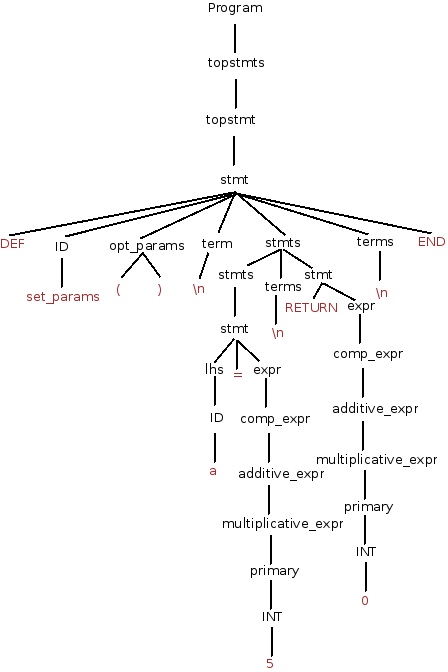
\includegraphics[width=0.8\textwidth]{Diagramme1.png}
\caption{arbre de dérivation}
\end{figure}


\subsection{Les modifications apportées sur la grammaire}
\subsubsection*{Au niveau des conditionnelles avec \emph{if} :}
Nous avons ajouter les lignes suivantes pour pouvoir traiter les conditionnelles sans \emph{``then''} : \\

\noindent stmt $\rightarrow$ IF expr stmts terms END \\
|IF expr stmts terms ELSE stmts terms END \\ 

\subsubsection*{Au niveau des conditionnelles avec \emph{unless} :}
Nous avons ajouter les lignes suivantes pour implémenter les conditionnelles avec \emph{``unless''} (fonctionnalité facultative) : \\

\noindent stmt $\rightarrow$ UNLESS expr THEN stmts terms END \\ 
| UNLESS expr THEN stmts terms ELSE stmts terms END \\
| UNLESS expr stmts terms END \\
| UNLESS expr stmts terms ELSE stmts terms END \\ 

\section{Conception}

\subsection{Les symboles} 


\subsubsection*{Structure}
Une table de symboles doit stocker un nombre important de noms de variables et d'informations qui leurs sont reliées. Elle n'a pas donc de taille fixe. De plus, il faut pouvoir y accéder de manière rapide. D'où le choix d'une liste chaînée.\\
 
Un symbole est caractérisé par son type, sa valeur (son contenu) et la table dans la quelle il se trouve. Celui-ci peut être soit un identifiant, soit un opérateur, soit une valeur (entier, réel ou chaîne de caractères). Pour cela, nous avons commencé par définir un type énuméré pour désigner le type du symbole de la manière suivante : 
\begin{verbatim} 
enum NodeEnume {TYPE_CONTENT, TYPE_INDEX, TYPE_OP}; 
\end{verbatim}
où : 
\begin{itemize}
\item \emph{TYPE$\_$CONTENT} pour une valeur (exemple : 5, 16.3 etc...) \\
\item \emph{TYPE$\_$INDEX} pour un identifiant (exemple : id, @x, etc...) \\
\item \emph{TYPE$\_$OP} pour un opérateur (exemple : if, while, then, end, +, $\times$, etc...) \\
\end{itemize}

Pour le contenu d'une variable, nous avons défini un type énuméré \emph{content} vu que le type du contenu peut être soit \textbf{int}, \textbf{float}, \textbf{string} ou \textbf{boolean} :
\begin{verbatim}
union content {
int e;
float f;
char* s;
int b;
}
\end{verbatim}
La dernière variable b désigne le contenu d'un booléen : elle prend 1 si c'est vrai, 0 sinon. \\

Un symbole est donc représenté sous la forme d'une structure de la manière suivante:  
\begin{verbatim}
struct Node { 
NodeEnum type; 
int valuetype; 
Content content; 
int index; 
OpNode op;
};
\end{verbatim}

avec :
\begin{itemize}
\item \emph{valuetype} est égal à :
\begin{itemize}
\item 0 pour \emph{int} 
\item 1 pour \emph{float} 
\item 2 pour \emph{string}
\item 3 pour \emph{boolean}
\item -1 pour \emph{undefined}
\end{itemize}
\item \emph{index} est le numéro du symbole dans la table. Cela permet de le retrouver facilemnt. 
\item \emph{op} est la structure de la table des symboles. 
\end{itemize}

\subsubsection*{Actions sur les symboles}
Les actions réalisées sur les symboles ont pour but de créer, initialiser et afficher un symbole : \\
\begin{itemize}
\item NewNodeInt (int) $\rightarrow$ Node* : cette fonction crée un nouveau symbole ayant une valeur de type entier. De la même manière, nous avons implémenté les fonctions \emph{NewNodeFloat, NewNodeBoolean, NewNodeString} et \emph{NewNodeVide}.
\item NodeFree (Node*) $\rightarrow$ void
\item NodePrint(Node*) $\rightarrow$ void
\item opr$\_$node (int type, char opr, Node*a, Node* b) $\rightarrow$ Node* : effectue l'opération \emph{opr} entre les deux symboles a et b.
\end{itemize}


\subsection{La table des symboles}
\begin{verbatim}
struct OpNode {
int name;
int num;
Node* node[1];
}
\end{verbatim}

\begin{itemize}
\item \emph{name}
\item \emph{num}
\item \emph{node}
\end{itemize}

\begin{figure}[!h]
\centering
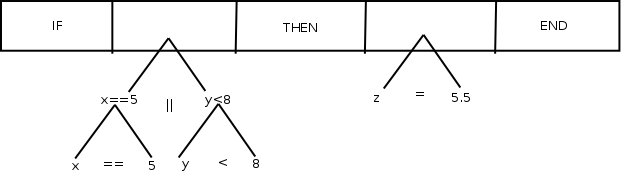
\includegraphics[width=0.8\textwidth]{exemple.png}
\caption{exemple}
\end{figure}

\section{Analyse sémantique}
L'analyse sémantique permet d'analyser et d'identifier les différents mots du langage. De plus, elle permet de vérifier que les types des différentes variables utilisées dans le programme sont corrects. Pour traiter cette phase, nous avons défini une table de symboles.
 

\subsection{Table des symboles}

\begin{center}
\begin{tabular}{|c|c|c|c|c|}
  \hline
  + & I & F & S & B \\
  \hline
  I & I & F &   &  \\
  \hline
  F & F & F &   & \\
  \hline
  S &   &   & S & \\
  \hline
  B & & & & \\
  \hline
\end{tabular}
\end{center}


\begin{center}
\begin{tabular}{|c|c|c|c|c|}
  \hline
  * & I & F & S & B \\
  \hline
  I & I & F &   &  \\
  \hline
  F & F & F &   & \\
  \hline
  S &   &   &  & \\
  \hline
  B & & & & \\
\hline
\end{tabular}
\end{center}



\begin{center}
\begin{tabular}{|c|c|c|c|c|}
  \hline
  cmp & I & F & S & B \\
  \hline
  I & B & B &   &  \\
  \hline
  F & B & B &   & \\
  \hline
  S &   &   & B  & \\
  \hline
  B & & & & \\
\hline
\end{tabular}
\end{center}


\subsection{Table des expressions}

\section{Production du code}

La génération du code intermédiaire du compilateur LLVM se fait sous forme de fichier texte. Le code assembleur LLVM est structurée en fonctions et utilise des variables locales préfixées par \% et des variables globales préfixées par @. Les types utilisés sont \textbf{i32} pour un entier et \textbf{float}. \\

\subsection{Traitement des instructions arithmétiques et logiques}
Toute construction d'expression du langage est associée à une expression sémantique où un registre est créé pour contenir le résultat de l'évaluation d'une sous-expression. \\

\noindent \textbf{Exemple :} \\
l'expression (9+8) $\times$ (7-3) est traduite comme suit :
\begin{verbatim}
%r1 = sub i32 7, 3 
%r2 = add i32 9, 8 
%r3 = mul i32 %r2, %r1 
\end{verbatim}

\subsection{Traitement des conditionnelles}
\subsection{Traitement des boucles \emph{for} et \emph{while}}



\section{Tests}


\newpage
\section*{Conclusion}
Au cours de ce projet, nous avons pu mettre en oeuvre les connaissances acquises au cours des séances de cours et de TD et les concepts élémentaires de compilation de langage de programmation. \\

Nous nous sommes familiarisées avec des outils d'analyse lexicale tel LEX et d'analyse syntaxique tel YACC.


\end{document}
